\def \Res {\operatorname{Res}}

\chapter{Residui}

\section{Residuo e residuo a infinito}

\begin{theorem}[Teorema dei Residui]
  Sia $\Omega \subset \C$ aperto con $z_1, \cdots, z_n \in \Omega$ e $f \in
  \mathcal{O}(\Omega')$ con $\Omega' = \Omega \setminus \left\{ z_1,\cdots, z_n
  \right\}$. Sia $\gamma$ una catena di curve chiuse in $\Omega$ tale che
  $\image(\gamma) \cap \left\{ z_1, \cdots,z_n \right\} = \varnothing$ e $\gamma
  \sim_\Omega 0$. Allora vale 
  \begin{equation*}
    \int_\gamma f(z)\ dz = 2 \pi i \sum_{i=1}^{n} \Ind_\gamma(z_i)
    \Res_{z_i}(f)
  \end{equation*}
  \label{thr:teorema_dei_residui}
\end{theorem}
\begin{proof}
  Supponiamo che $\gamma = \sum_{i=1}^n \Ind_\gamma (z_i) \gamma_i$, allora
  per il Teorema di Cauchy \ref{thr:formule-di-cauchy-generale} vale 
  \begin{equation*}
    \int_\gamma f(z) \ dz = \sum_{i = 1}^{n} m_i \int_{\gamma_i} f(z) \ dz
    = \sum_{i=1}^n \Ind_\gamma(z_i) \Res_{z_i}(f)
  \end{equation*}
\end{proof}

\begin{definition}
  Si dice che $\Omega \subset \C$ è un \textbf{intorno aperto di $\infty$} se
  è un aperto contenente il complemente di un insieme limitato di $\C$. Se $f
  \in \mathcal{O}(\Omega)$ si dice che $f$ ha una \textbf{singolarità isolata
  all'infinito} se la funzione $g(w) = f(1/w)$ ha una singolarità isolata a $w
  = 0$. Il tipo di singolarità per $f$ in $\infty$ è lo stesso per $g$ in $0$.
  Se $0$ è elimiminabile per $g$ allora si dice che $f$ è \textbf{olomorfa
  all'inifito}. Il \textbf{residuo all'infinito} di $f$ è 
  \begin{equation*}
    \Res_\infty(f) = \Res_0\left( -\frac{g(w)}{w^2} \right)
  \end{equation*}
  \label{def:varie_definizioni_all'inifinito}
\end{definition}

\begin{lemma}
  Sia $f \in \mathcal{O}(\Omega)$ con $\C \setminus B_0(R) \subset \Omega$.
  Allora 
  \begin{equation*}
    \Res_\infty (f) = -\frac{1}{2\pi i } \int_{\gamma_R} f(z)\ dz
  \end{equation*}
  \label{lem:residuo_a_infinito}
\end{lemma}
\begin{proof}
  Sia $g(w) = f(1/w)$. Allora il residuo a infinito di $f$ è uguale a 
  \begin{equation*}
    \Res_\infty(f) = \Res_0\left(-\frac{g(w)}{w^2}  \right) = \int_{\gamma}
    -\frac{g(w)}{w^2}\ dw
  \end{equation*}
  dove con $\gamma \coloneqq e^{-it}/R$. Percorrendola in senso antiorario,
  indichiamo questa curva con $-\gamma$, allora
  \begin{equation*}
    \int_{\gamma} -\frac{g(w)}{w^2}\ dw  = - \int_{0}^{2\pi}
    \frac{g(\gamma(t))}{\gamma(t)^2} \gamma'(t)\ dt 
  \end{equation*}
  osservando che $-1/\gamma_R = \gamma$ otteniamo che 
  \begin{align*}
     \int_{0}^{2\pi} -\frac{g(\gamma(t))}{\gamma(t)^2} \gamma'(t)\ dt
     & = \int_{0}^{\pi} f(\gamma_R(t)) \gamma'_R(t) \ dt\\
     & = \int_{\gamma_R} f(z)\ dz
  \end{align*}
  ovvero la tesi.
\end{proof}

\begin{corollary}
  Sia $f \in \mathcal{O}(\C \setminus \left\{ z_1, \cdots, z_n \right\}$. Allora 
    \begin{equation*}
      \Res_\infty(f) = - \sum_{i=1}^{n} \Res_{z_i}(f) = 0
    \end{equation*}
\end{corollary}
\begin{proof}
  Basta integrale lungo una circonferenza $\gamma$ con $z_1, \cdots, z_n$ punti
  interni e applicare il Teorema dei residui \ref{thr:teorema_dei_residui}.
\end{proof}


\section{Calcolo dei residui}

\begin{lemma}
  Sia $f$ una un polo semplice in $z_0$, ovvero di ordine $1$, e $g$ funzione 
  olomorfa in un intorno di $z_0$, allora $\Res_{z_0}(fg) = g(z_0) \Res_{z_0}(f)$.
  \label{lem:calcolo_residuo_prodotto_funz}
\end{lemma}
\begin{proof}
  Sia $f(z) = a_{-1}(z-z_0)^{-1} + h(z)$ con $h$ olomorfa vicino a $z_0$. Sia
  $g(z) = b_0 + h_1(z) (z-z_0)$ con $h_1$ olomorfa vicino a $z_0$. Allora
  \begin{equation*}
    f(z)g(z) = \frac{a_{-1}b_0}{z-z_0} + \left(a_{-1}h_1(z) + b_0h(z)
    + h(z)h_1(z)(z-z_0)\right)
  \end{equation*}
  Notiamo che dal secondo membro in poi è una funzione olomorfa in un
  intorno di $z_0$, vale quindi che la sua serie di Laurent è una serie di 
  potenze. Pertanto il residuo in $z_0$ dev'essere
  \begin{equation*}
    \Res_{z_0}(fg) = a_{-1}b_0 = a_{-1}g(z_0)
  \end{equation*}
\end{proof}

\begin{corollary}
  Se $f$ ha uno zero semplice all'infinito allora 
  \begin{equation*}
    \Res_\infty(f) = - \lim_{z \to +\infty} z f(z)
  \end{equation*}
  \label{cor:calcolo_residuo_infinito}
\end{corollary}
\begin{proof}
  Sia $g(w) = f(1/w)$. Allora sia $\hat{g}(w) = w h(w)$ l'estensione olomorfa di
  $g$ (infatti $g$ ha un polo semplice in $w = 0$ per ipotesi), con $h(0) \neq 0$. 
  Quindi $g(w)/w^2 = h(w)/w$ per ogni $w \neq 0$ allora $g(w)/w^2$ ha un polo 
  semplice in $0$. Per il Lemma \ref{lem:calcolo_residuo_prodotto_funz} vale 
  \begin{align*}
    \Res_\infty(f) & = \Res_0\left( -\frac{g(w)}{w^2} \right)
    = \Res_0\left(-\frac{1}{w} h(w)\right) \\
    & = h(0) \Res_0 \left( -\frac{1}{w} \right) \\
    & = - \lim_{w \to 0} \frac{g(w)}{w} \\
    & = - \lim_{z \to 0} z f(z)
  \end{align*}
\end{proof}

\begin{lemma}
  Se $f$ è olomorfa nell'intorno di $z_0$ e in $z_0$ ha uno zero semplice allora
  $1/f$ ha un polo semplice in $z_0$ e vale 
  \begin{equation*}
  \Res_{z_0}\left( \frac{1}{f} \right) = \frac{1}{f'(z_0)}
  \end{equation*}
  \label{lem:calcolo_residuo_zero_semplice_inversa}
\end{lemma}
\begin{proof}
  Poiché $f$ ha uno zero semplice, vale $f(z) = (z-z_0) g(z)$ con $g$ olomorfa
  in un intorno di $z_0$ e $g(z_0) = f'(z_0) \neq 0$. Quindi 
  \begin{equation*}
    \frac{1}{f(z)} = \frac{1}{z-z_0} \frac{1}{g(z)}
  \end{equation*}
  con $1/g$ olomorfa vicino a $z_0$. Per il Lemma
  \ref{lem:calcolo_residuo_prodotto_funz} vale
  \begin{equation*}
    \Res_{z_0}\left(\frac{1}{f}\right) = \Res_{z_0}\left(\frac{1}{z-z_0}\right) 
                        \frac{1}{g(z_0)}
  \end{equation*}
  poiché $\Res_{z_0} 1/(z-z_0) = 1$ vale la tesi, ovvero 
  \begin{equation*}
    \Res_{z_0}\left(\frac{1}{f}\right) = \frac{1}{g(z_0)}
    = \frac{1}{f'(z_0)}
  \end{equation*}
\end{proof}

\begin{lemma}
  Se $f$ ha un polo di ordine $m$ in $z_0$ allora 
  \begin{equation*}
    \Res_{z_0}(f) = \frac{1}{(m-1)!} \lim_{z \to z_0} ((z-z_0)^m
  f(z))^{(m-1)}
  \end{equation*}
  \label{lem:calcolo_residuo_polo}
\end{lemma}
\begin{proof}
  Sia $g(z) = (z-z_0)^m f(z)$ allora questa è l'estensione olomorfa della
  funzione $f$ che avrà serie di Laurent della forma
  \begin{equation*}
    g(z) = \sum_{n = 0}^{+\infty} b_n(z-z_0)^n
  \end{equation*}
  Per cui la serie di Laurent di $f$ diventa
  \begin{equation*}
    f(z) = b_0(z-z_0)^{-m} + \cdots + b_{m-1}(z-z_0)^{-1} + \cdots
  \end{equation*}
  allora 
  \begin{equation*}
    a_{-1} = \Res_{z_0}(f) = b_{m-1} = \frac{g^{(m-1)}(z_0)}{(m-1)!}
  \end{equation*}
  da cui la tesi.
\end{proof}

\begin{example}
  \begin{enumerate}
    \item Calcoliamo i residui della funzione $h(z) = z^2 / (z^2 - 1)$, allora $h
        \in \mathcal{O}(\C \setminus \left\{ \pm 1 \right\}$ e vale la seguente
         decomposizione
         \begin{equation*}
            h(z) = \frac{1}{z-1} \frac{z^2}{z+1} = f(z)g(z)
         \end{equation*}
         Quindi 
         \begin{enumerate}
            \item In $z = 1$, la funzione $f$ ha un polo semplice con residuo $1$ e $g$
                è olomorfa in un intorno di $1$ quindi 
                \begin{equation*}
                    \Res_1(h) = g(1) \Res_1(f) = \frac{1}{2}
                \end{equation*}
            \item In $z = -1$, la funzione $g$ ha un polo semplice con residuo $1$
                mentre $f$ è olomorfa in un intorno di $-1$ quindi 
                \begin{equation*}
                    \Res_{-1}(h) = f(-1) \Res_{-1}(g) = - \frac{1}{2}
                \end{equation*}
            \item All'infinito vale 
                \begin{equation*}
                    \Res_\infty(h) = - \Res_{1}(h) - \Res_{-1}(h) = 0
                \end{equation*}
         \end{enumerate}
       \item Calcoliamo i residui di $h(z) = 1/ \sin(z)$. La funzione si annulla
         solo in $z = k\pi$ con $k \in \Z$ e vale $\sin(z)' = \cos(z) \neq 0$
         per $z \in k \pi$. Quindi sono poli semplici e per il Lemma
         \ref{lem:calcolo_residuo_zero_semplice_inversa} allora vale 
         \begin{equation*}
           \Res_{k\pi}(h) = \frac{1}{\cos(k\pi)} = \pm 1
         \end{equation*}
         con $1$ se $k$ pari e $-1$ se $k$ dispari.
       \item Consideriamo la funzione 
         \begin{equation*}
           h(z) = \frac{z^2}{z^3 - z^2 - z + 1} = \frac{z^2}{(z-1)^2(z+1)}
         \end{equation*}
         allora $h \in \mathcal{O}(\C \setminus \left\{ \pm 1 \right\}$ e 
           \begin{enumerate}
             \item Se $z = 1$ il polo è doppio quindi 
               \begin{equation*}
                 \Res_1(h) = \left(\frac{z^2}{z+1}\right)'|_{z = 1} = \frac{3}{4}
               \end{equation*}
             \item Se $z = -1$ il polo di ordine $1$ quindi
               \begin{equation*}
                 \Res_{-1}(h) = \frac{(-1)^2}{(-1-1)^2} = \frac{1}{4} 
               \end{equation*}
             \item Invece a infinito diventa 
               \begin{equation*}
                 \Res_\infty(h) = - \frac{3}{4} - \frac{1}{4} = -1
               \end{equation*}
           \end{enumerate}
  \end{enumerate}
\end{example}


\section{Applicazioni dei residui agli integrali reali}

Dividiamo l'argomento in due casi. Il primo caso è quello in cui
$\morphism{f}{\C}{\C}$ ristretto all'asse reale non presenta singolarità. Il
secondo caso è quello in cui $f|_\R$ ha delle singolarità di qualche tipo.

\begin{proposition}[Caso I]
  \label{prop:caso-i}
  Consideriamo $\morphism{f}{\R}{\R}$ una funzione reale continua, intesa come
  restrizione di $g \in \mathcal{O}(\Omega \setminus \left\{ z_1, \cdots,z_n
  \right\})$ e con $\Im(z_1), \cdots,\Im(z_n) > 0$ e $\Omega \supset \left\{
  z \in \C \,\middle|\, \Im(z) \ge 0 \right\}$. Se esistono $K,M > 0$ e $a > 0$ 
  tali che 
  \begin{equation*}
    |f(z)| \le \frac{K}{|z|^{1+a}}
  \end{equation*}
  per $|z| \ge M$, allora vale
  \begin{equation}
    \label{eq:integrale_improprio_no_poli_reali}
    \int_{-\infty}^{+\infty} f(x)\ dx = 2\pi i \sum_{i=1}^{n} \Res_{z_i}(f)
  \end{equation}
\end{proposition}
\begin{proof}
   Per $x \in \R$ vale $|f(x)| \le K/|x|^{1+a}$ che è integrabile su $(-\infty,
  \alpha)$ e su $(\beta, +\infty)$ per ogni $\alpha < 0$ e $\beta > 0$. Quindi
  esistono i limiti 
  \begin{align*}
    \lim_{R\to +\infty} \int_{-R}^{\alpha}f(x)\ dx &= L^+ \in \R \\
    \lim_{R \to +\infty} \int_{\beta}^{R} f(x)\ dx &= L^- \in \R 
  \end{align*}
  e quindi esiste il limite
  \begin{equation*}
    \int_{-\infty}^{+\infty}f(x)\ dx = \lim_{R\to+\infty} \int_{-R}^R f(x) \ dx
  \end{equation*}
  Per dimostrare la formula applichiamo il Teorema dei Residui a $f$ lungo la
  catena $\Gamma$ ottenuta come in Figura \ref{fig:residui_1}. 
  \begin{figure}[h]
    \centering
    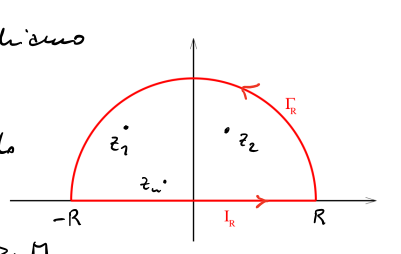
\includegraphics[width=0.5\linewidth]{images/analisi_complessa/residui_figura_1.png}
    \caption{Integrazione lungo curva}
    \label{fig:residui_1}
  \end{figure}
  Quindi otteniamo 
  \begin{equation*}
    2 \pi i \sum_{i=1}^{n} \Res_{z_i}(f) = \int_{I_R} f(z)\ dz + \int_{\Gamma_R}
    f(z)\ dz
  \end{equation*}
  il secondo integrale osserviamo che 
  \begin{equation*}
    \left|\int_{\Gamma_R} f(z)\ dz \right| \le
    \frac{K}{R^{1+a}}\mathcal{H}^{1}(\Gamma_R) = \frac{\pi K}{R^{a}}
  \end{equation*}
  e quindi tende a $0$ per $R \to +\infty$. Mentre il primo integrale
  corrisponde all'integrale improprio che volevamo calcolare. Da cui
  \begin{equation*}
     \int_{-\infty}^{+\infty} f(x)\ dx = 2\pi i \sum_{i=1}^{n} \Res_{z_i}(f)
  \end{equation*}  
\end{proof}

\begin{proposition}[Caso II]
	\label{prop:caso-ii}
    Sia $\morphism{f}{\R}{\R}$ una funzione reale continua, resitrizione di una
    funzione complessa $g \in \mathcal{O}(\Omega \setminus \left\{ z_1, \cdots,
    z_n\right\}$ e con $\Omega \supset \left\{ z \in \C \,\middle|\, \Im(z) \ge
    0\right\}$ e $z_1, \cdots, z_n \in \left\{ z \in \C \,\middle|\, \Im(z)
    > 0 \right\}$. Se esistono $K,M > 0$ tali che 
    \begin{equation*}
      |f(z)| \le \frac{K}{|z|}
    \end{equation*}
    allora vale 
    \begin{equation*}
      \int_{-\infty}^{+\infty} f(x) e^{ix} \ dx = 2\pi i \sum_{i=1}^n
      \Res_{z_i}(f(z) e^{iz})  
    \end{equation*}
\end{proposition}
\begin{proof}
    Essenzialmente ci ritroviamo a usare il Teorema dei Residui in modo analogo
    al caso I, solo che questa volta considereremo un quadrato dato che abbiamo
    anche la parte complessa della funzione $f$. Infatti possiamo riscrivere
    l'integrale come segue:
    \begin{equation*}
      \int_{-\infty}^{+\infty} f(x) e^{ix}\ dx = \int_{-\infty}^{+\infty}
      f(x)\cos(x) \ dx + i\int_{-\infty}^{+\infty} f(x)\sin(x)\ dx
    \end{equation*}
    Integriamo lungo il quadrato $\Gamma_{A,B}$ descritto in 
    Figura \ref{fig:residui_funz_fourier}
    
    \begin{figure}[h]
      \centering
      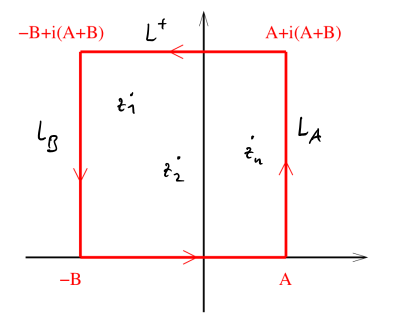
\includegraphics[width=0.4\linewidth]{images/analisi_complessa/residui_figura_2.png}
      \caption{Visualizzazione delle curve di integrazione}
      \label{fig:residui_funz_fourier}
    \end{figure}

    Spezziamo quindi l'integrazione sul quadrato nei suoi quattro lati,
    e mostriamo che l'integrale su $L_B, L_A, L^+$ tendono a $0$ per $A,B \to
    +\infty$. Scegliamo $A,B \ge M$, in maniera tale da poter poi limitare la
    funzione $f$. Prendiamo quindi il caso di $L^+$ che parametriziamo con la 
    curva $\gamma^+(x) = -x + i(A+B)$. Allora
    \begin{align*}
      \left| \int_{\gamma^+} f(z)e^{iz}\ dz  \right| & = \left| \int_{-A}^B f(-x
      + i(A+B)) (-e^{-ix - (A+B)}\ dx\right| \\
        & \le \frac{K}{T}e^{-(A+B)} \mathcal{H}^1(\gamma^+) = Ke^{-(A+B)}
    \end{align*}
    l'ultima disuguaglianza dipende dal fatto che $|f(z)| \le K/(A+B)$ per $|z| \ge
    (A+B) \ge M$. \\

    Consideriamo ora il caso del lato $L_A$, parametrizzato dalla curva
    $\gamma_A(y) = A + iy$, allora
    \begin{equation*}
      \left|\int_{\gamma_A} f(z) e^{iz}\right| 
      = \left|\int_{0}^{A+B} f(A+iy)e^{-y + iA}i \ dy \right| 
      \le \frac{K}{A} \int_{0}^{A+B} e^{-y}\ dy
    \end{equation*}
    e questo ovviamente tende a $0$ per $A+B \to +\infty$.\\
    Quindi per il Teorema dei Residui
    \begin{equation*}
      2 \pi i \sum_{i=1}^n \Res_{z_i} (f) = \int_{\Gamma_{A,B}} f(z)e^{iz}\ dz 
    \end{equation*}
    e il membro di destra ha come solo sopravvissuto 
    \begin{equation*}
      \int_{\Gamma_{A,B}} f(z)e^{iz}\ dz = \int_{A}^{B} f(z)e^{iz}\ dz \quad\
      \text{per}\ A+B \to 0
    \end{equation*}
    da cui vale la tesi.
\end{proof}

\begin{proposition}[Caso III]
  
  \begin{figure}[h]
    \centering
    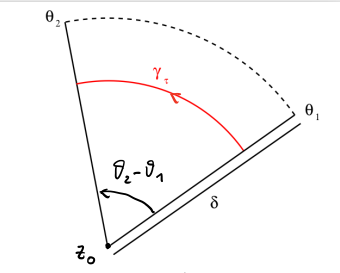
\includegraphics[width=0.4\linewidth]{images/analisi_complessa/residui_figura_3.png}
    \caption{Descrizione delle ipotesi}
  \end{figure}

  Sia $\Omega$ aperto e $z_0 \in \Omega$ e $f \in
  \mathcal{O}(\Omega\setminus\left\{ z_0 \right\})$. Sia
  $\overline{B_{z_0}}(\delta) \subset \Omega$ e sia $\gamma_\tau$ l'arco di
  raggio $\tau$ con $\theta_1 \le \operatorname{arg}(\gamma_\tau) \le \theta_2$
  e $\tau \le \delta$. Se $f$ ha un polo semplice o una singolarità eliminabile
  in $z_0$ allora vale
  \begin{equation*}
    \lim_{\tau \to 0} \int_{\gamma_{\tau}} f(z) \ dz = ib(\theta_2-\theta_1)
  \end{equation*}
  \label{prop:caso-iii}
\end{proposition}
\begin{proof}
  Possiamo riscrivere 
  \begin{equation*}
    f(z) = \frac{b}{z-z_0} + h(z)
  \end{equation*}
  con $h$ olomorfa in un intorno di $z_0$. Quindi
  \begin{equation*}
    \int_{\gamma_\tau} f(z)\ dz = \int_{\theta_1}^{\theta_2}
    \frac{b}{\tau e^{i\theta}} i \tau e^{i\theta} \ d\theta + \int_{\gamma_\tau}
    h(z)\ dz
  \end{equation*}
  per cui mostriamo che il secondo integrale converge a $0$ in modulo, ovvero
  \begin{equation*}
    \left| \int_{\gamma_\tau} h(z)\ dz \right| \le \max_{\gamma_\tau} |h|
    \mathcal{H}^1(\gamma_\tau) 
  \end{equation*}
  ma la lunghezza di $\gamma_\tau\to 0$ per $\tau \to 0$, quindi tutto
  l'integrale tende a $0$.
  Per cui
  \begin{equation*}
    \lim_{\tau\to 0} \int_{\gamma_\tau} f(z)\ dz = \lim_{\tau \to 0} 
    \int_{\theta_1}^{\theta_2} \frac{b}{\tau e^{i\theta}} i \tau e^{i\theta}
    \ d\theta \to ib(\theta_2 - \theta_1) 
  \end{equation*}
\end{proof}

\begin{proposition}[Caso IV - Funzioni razionali]
  \label{prop:caso-iv}
  Siano $g,h$ polinomi reali in $x,y$ con $h \neq 0$ per $x^2 + y^2 = 1$. Allora
  possiamo definire la funzione razionale 
  \begin{equation*}
    Q(x,y) \coloneqq \frac{g(x,y)}{h(x,y)} 
  \end{equation*}
  e vale la seguente formula
  \begin{equation*}
    \int_0^{2\pi} Q(\cos(\theta), \sin(\theta)) \ d\theta = 2\pi
    i \sum_{i=1}^n \Res_{z_i} (f)
  \end{equation*}
  dove 
  \begin{equation*}
    f(z) \coloneqq \frac{1}{iz} Q\left( \frac{z+z^{-1}}{2},
    \frac{z-z^{-1}}{2i} \right)
  \end{equation*}
\end{proposition}
\begin{proof}
  Consideriamo il cerchio centrato nell'origine e di raggio $1$, parametrizzato
  dalla curva $\gamma = \partial B_0(1) = e^{i\theta}$ (con $\theta \in \left[
  0,2\pi \right]$). Allora
  \begin{equation*} 
    f(e^{i\theta}) = \frac{1}{ie^{i\theta}}
    Q\left(\cos(\theta),\sin(\theta)\right)
  \end{equation*}
  e quindi 
  \begin{equation*}
    \int_{\gamma} f(z) \ dz = \int_{0}^{2\pi} Q(\cos(\theta), \sin(\theta))\
    d\theta
  \end{equation*}
  e infine per il Teorema dei Residui si ottiene la tesi.
\end{proof}

\begin{example}
  \begin{enumerate}
    \item Calcoliamo 
      \begin{equation*}
        I = \int_{0}^{+\infty} \frac{1}{(1+x^2)^2}\ dx = \int_{0}^{+\infty}
        f(x)\ dx
      \end{equation*}
      possiamo vedere che la funzione è pari, quindi 
      \begin{equation*}
        2I = \int_{-\infty}^{+\infty} \frac{1}{(1+x^2)^2}\ dx
      \end{equation*}
      inoltre mostriamo che $f(z)$ è limitata. Quindi 
      \begin{equation*}
        |f(z)| = \left|\frac{z^{-4}}{(z^{-2}+1)^2}\right|
        = \frac{|z|^{-4}}{|z^{-2}+1|^2} \le \frac{1}{z^{4}(1-M^2)^2}
      \end{equation*}
      con $|z| \ge M > 1$. Quindi la funzione è limitata a infinito. Calcoliamo
      infine i residui di $f$ in $\pm i$, ma solo uno dei poli sta nel
      semispazio $\Im(i) > 0$. Quindi dalla formula
      \eqref{eq:integrale_improprio_no_poli_reali} risulta
      \begin{equation*}
        2I = 2\pi i \Res_{i}(f) = 2\pi i \frac{1}{4i} = \frac{\pi}{2}
      \end{equation*}
    \item Proviamo a calcolare 
      \begin{equation*}
        I = \int_{-\infty}^{+\infty} \frac{\cos(x)}{1+x^2}\ dx  
      \end{equation*}
      definiamo $f(z) = 1/(1+z^2)$ allora questa risulta limitata in modulo
      a infinito. Inoltre possiamo vedere che l'integrale $I$ è 
      \begin{equation*}
        I = \Re\left( \int_{-\infty}^{+\infty} \frac{e^{ix}}{1+x^2} \ dx\right)
      \end{equation*}
      ovvero possiamo riscrivere per quanto visto nella Proposizione \ref{prop:caso-ii} che 
      \begin{equation*}
        I = \Re\left( 2\pi i \Res_{i} \left(\frac{e^{iz}}{1+z^2} \right) \right)
      \end{equation*}
      e poiché il residuo è $e^{-1}/2i$ si ottiene 
      \begin{equation*}
        I = \Re\left( \pi e^{-1} \right) = \frac{\pi}{e}
      \end{equation*}
    \item Calcoliamo l'integrale seguente 
      \begin{equation*}
        I = \int_{-\infty}^{+\infty} \frac{\sin(x)}{x}\ dx
      \end{equation*}
      Allora possiamo vedere che ha una singolarità in $0$, definiamo $f(z)
      = 1/z$ e la curva $\Gamma$ come in figura 
      \begin{figure}[h]
        \centering
        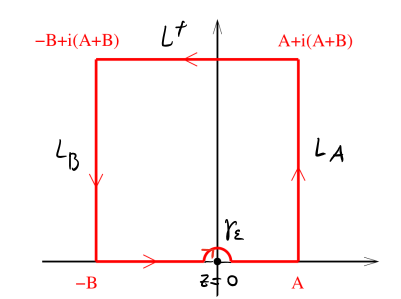
\includegraphics[width=0.4\linewidth]{images/analisi_complessa/residui_figura_4.png}
        \caption{Visualizzazione della curva $\Gamma$}
      \end{figure}
      Allora possiamo risolvere come nel caso II ma dobbiamo spezzare
      l'integrale in $3$ curve:
      \begin{equation*}
        \int_{-\infty}^{-\varepsilon} \frac{e^{ix}}{x}\ dx +
        \int_{\gamma_\varepsilon} \frac{e^{iz}}{z}\ dz +
        \int^{+\infty}_{+\varepsilon} \frac{e^{ix}}{x}\ dx
        \overset{\text{Thr. Cauchy}}{=} 0
      \end{equation*}
      per ogni $\varepsilon > 0$, ma preso sufficientemente piccolo. Per la
      Proposizione \ref{prop:caso-iii} prendiamo $\theta_1 = \pi$ e $\theta_2 = 0$ e $b
      = \Res_{0}(e^{iz}f(z)) = 1$. Allora abbiamo che per $\varepsilon \to 0$
      \begin{equation*}
        \int_{\gamma_\varepsilon} \frac{e^{iz}}{z}\ dz = - \pi i
      \end{equation*}
      e di conseguenza abbiamo che 
      \begin{equation*}
        \int_{-\infty}^{-\varepsilon} \frac{e^{ix}}{x}\ dx
        + \int_{\varepsilon}^{+\infty} \frac{e^{ix}}{x}\ dx = \pi i
      \end{equation*}
      per $\varepsilon \to 0$. Quindi 
      \begin{equation*}
        I = \Im\left( \int_{-\infty}^{+\infty} \frac{e^{ix}}{x}\ dx \right)
        = \Im(\pi i ) = \pi
      \end{equation*}
    \item Proviamo a calcolare invece l'integrale 
      \begin{equation*}
        I = \int_{0}^{2\pi} \frac{d\theta}{3-\cos(\theta)}
      \end{equation*}
      Possiamo vederlo come un integrale di un polinomio composto con $\cos,
      \sin$, quindi $Q(x,y) = 1/(3-x)$. Allora per la Proposizione
      \ref{prop:caso-iv}
      \begin{equation*}
        f(z) = \frac{1}{iz} \frac{1}{3 - \frac{z+z^{-1}}{2}}
        = \frac{1}{z-3+2\sqrt{2}} \frac{2i}{z-3-2\sqrt{2}}
      \end{equation*}
      Quindi calcoliamo solo il residuo in $z_1 = 3-2\sqrt{2}$, 
      dato che è l'unica singolarità che è all'interno di $B_0(1)$. Per cui
      \begin{equation*}
        \Res_{z_1}(f) = \frac{i}{2\sqrt{2}}
      \end{equation*}
      e quindi si ottiene 
      \begin{equation*}
        I = 2\pi i \left( -\frac{i}{2\sqrt{2}} \right) = \frac{\pi}{\sqrt{2}}
      \end{equation*}
  \end{enumerate}
\end{example}
